\chapter{Direct Memory Access - DMA - implementation}
So far, the Programmable Logic (PL) and Processing System (PS) sections of the System on Module (SoM) have been utilized independently, without establishing a direct interconnection for communication or control. This project shifts the focus towards the development of a design that enables the system processor to interact with the programmable logic by reading from a specific memory address.

To achieve this, a dedicated component is implemented, which assigns a fixed memory address that supports read and write (R/W) operations. This enables seamless data exchange between the PL and PS, facilitating efficient communication. The key digital components utilized in this design include a register and a First-In, First-Out (FIFO) memory, both of which help manage data flow between the programmable logic and the processor. In addition, also the Direct Memory Access (DMA) has been exploited. The DMA is a feature in computer systems which allows hardware components to directly accessing the system memory without involving the CPU for every transfer. The data transfer is managed by a DMA controller, which is initially set by the CPU. This type of communication is used in embedded systems, high-speed networking, and storage devices to optimize performance. 

\section{Vivado project}
As far as the creation of the Vivado project is concerned, all the steps needed to derive the final block scheme are omitted since they follow the same steps described in the previous chapters. In this section it is just shown the block design and a brief description of the blocks is given.
\begin{figure}[h!t!]
	\centering
	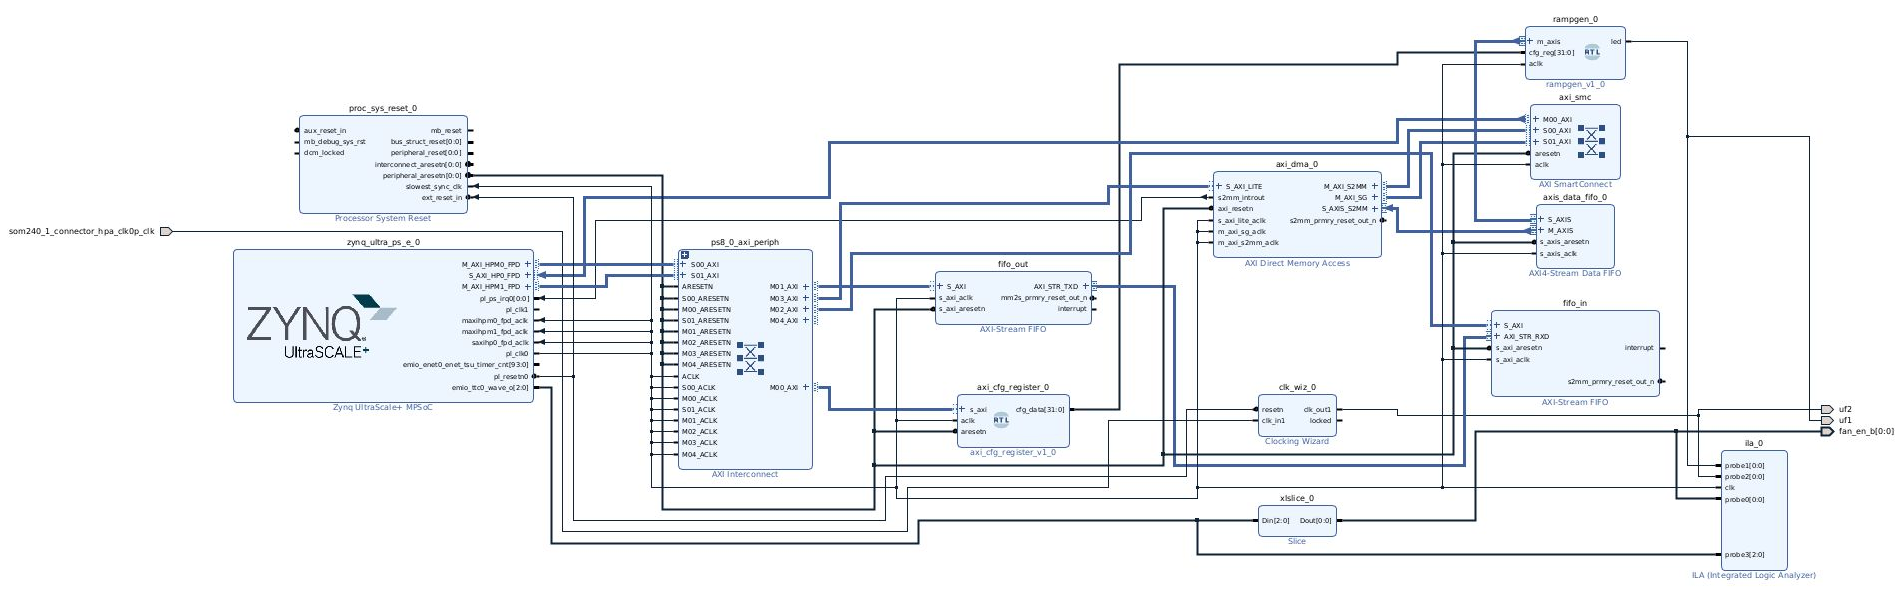
\includegraphics[width=1\textwidth]{images/dma}
	\caption{Vivado DMA block scheme.}
	\label{fig:dma}
\end{figure}
The block scheme is composed by the following blocks:
\begin{itemize}
	\item Zynq UltraScale+ Processing System: This is a highly versatile and powerful System-on-Chip (SoC) that combines programmable logic (FPGA fabric) and processing capabilities (ARM Cortex cores). It's the brain of the system, handling computation, decision-making, and coordination between other components.
	
	\item AXI Direct Memory Access (DMA): This block facilitates high-speed data transfer between memory and peripherals or other components, bypassing the CPU. It’s crucial for efficient data handling in high-performance systems.
	
	\item FIFO (First-In, First-Out): A type of data buffer used to ensure smooth and orderly data flow. It stores data temporarily and releases it in the same order it was received, preventing bottlenecks in the system.
	
	\item AXI Interconnect: This connects various AXI-based components within the design. It manages data flow between the processor, peripherals, memory, and other AXI-compatible blocks, ensuring efficient communication.
	
	\item Peripheral Interfaces: These are bridges connecting external devices (like sensors, displays, or communication modules) to the main system. They ensure compatibility and proper data exchange between the system and peripherals.
	
	\item Memory Controller: This manages the read and write operations to and from external or on-chip memory, ensuring data is stored and accessed efficiently.
\end{itemize}



\section{Petalinux project}
Despite having created the Vivado project and established a design flow, the current approach does not work in this case. The previous method was discovered through trial and error rather than a structured research effort like this one. The main issue arises during board boot: the DMA controller attempts to access memory addresses defined in the Vivado block design before the FPGA has been programmed. To address this, the device tree is modified after boot, creating a custom configuration to ensure proper memory access and system functionality. To upload the code relative to the DMA testing, there are few steps to follow:
\begin{itemize}
	\item The first step is to create the file \textbf{pl-<projectname>.dtsi}. The file has to be modified as shown in the following code. The node \textit{fragment@1} is copied from \textbf{pl.dtsi} (found in \textit{components/plnx\_workspace/device-tree/device-tree/}. In addition all the data relative to the DMA and the memory instantiation are copied. \textbf{dmatest\_0} has to be written anew instead, since it is not found in any file.
	\vspace{0.1cm}
	\begin{lstlisting}[language=C]
		/*
		* CAUTION: This file is automatically generated by Xilinx.
		* Version: XSCT
		* Today is: Wed Feb 26 13:53:04 2025
		*/
		
		
		/dts-v1/;
		/plugin/;
		/ {
			fragment@1 {
				target = <&amba>;
				overlay1: __overlay__ {
					#address-cells = <2>;
					#size-cells = <2>;
					afi0: afi0 {
						compatible = "xlnx,afi-fpga";
						config-afi = < 0 2>, <1 2>, <2 0>, <3 0>, <4 2>, <5 2>, <6 0>, <7 0>, <8 0>, <9 0>, <10 0>, <11 0>, <12 0>, <13 0>, <14 0xa00>, <15 0x000>;
					};
					clocking0: clocking0 {
						#clock-cells = <0>;
						assigned-clock-rates = <99999001>;
						assigned-clocks = <&zynqmp_clk 71>;
						clock-output-names = "fabric_clk";
						clocks = <&zynqmp_clk 71>;
						compatible = "xlnx,fclk";
					};
					clocking1: clocking1 {
						#clock-cells = <0>;
						assigned-clock-rates = <99999001>;
						assigned-clocks = <&zynqmp_clk 72>;
						clock-output-names = "fabric_clk";
						clocks = <&zynqmp_clk 72>;
						compatible = "xlnx,fclk";
					};
					
					dmatest_0: dmatest@0 {
						compatible ="xlnx,axi-dma-test-1.00.a";
						dmas = <&axi_dma_0 1>;
						dma-names = "dma0";
					};
					axi_cfg_register_0: axi_cfg_register@b0000000 {
						clock-names = "aclk";
						clocks = <&zynqmp_clk 71>;
						compatible = "xlnx,axi-cfg-register-1.0";
						reg = <0x0 0xb0000000 0x0 0x80>;
					};
					axi_dma_0: dma@a0020000 {
						#dma-cells = <1>;
						clock-names = "m_axi_s2mm_aclk", "m_axi_sg_aclk", "s_axi_lite_aclk";
						clocks = <&zynqmp_clk 71>, <&zynqmp_clk 71>, <&zynqmp_clk 71>;
						compatible = "xlnx,axi-dma-7.1", "xlnx,axi-dma-1.00.a";
						interrupt-names = "s2mm_introut";
						interrupt-parent = <&gic>;
						interrupts = <0 89 4>;
						reg = <0x0 0xa0020000 0x0 0x10000>;
						xlnx,addrwidth = <0x20>;
						xlnx,include-sg ;
						xlnx,sg-length-width = <0x17>;
						dma-channel@a0020030 {
							compatible = "xlnx,axi-dma-s2mm-channel";
							dma-channels = <0x1>;
							interrupts = <0 89 4>;
							xlnx,datawidth = <0x20>;
							xlnx,device-id = <0x0>;
						};
					};
					fifo_in: axi_fifo_mm_s@a0010000 {
						clock-names = "s_axi_aclk";
						clocks = <&zynqmp_clk 71>;
						compatible = "xlnx,axi-fifo-mm-s-4.3";
						reg = <0x0 0xa0010000 0x0 0x10000>;
						xlnx,axi-str-rxd-protocol = "XIL_AXI_STREAM_ETH_DATA";
						xlnx,axi-str-rxd-tdata-width = <0x20>;
						xlnx,axi-str-txc-protocol = "XIL_AXI_STREAM_ETH_CTRL";
						xlnx,axi-str-txc-tdata-width = <0x20>;
						xlnx,axi-str-txd-protocol = "XIL_AXI_STREAM_ETH_DATA";
						xlnx,axi-str-txd-tdata-width = <0x20>;
						xlnx,axis-tdest-width = <0x4>;
						xlnx,axis-tid-width = <0x4>;
						xlnx,axis-tuser-width = <0x4>;
						xlnx,data-interface-type = <0x0>;
						xlnx,has-axis-tdest = <0x0>;
						xlnx,has-axis-tid = <0x0>;
						xlnx,has-axis-tkeep = <0x0>;
						xlnx,has-axis-tstrb = <0x0>;
						xlnx,has-axis-tuser = <0x0>;
						xlnx,rx-cascade-height = <0x0>;
						xlnx,rx-enable-ecc = <0x0>;
						xlnx,rx-fifo-depth = <0x800>;
						xlnx,rx-fifo-pe-threshold = <0x5>;
						xlnx,rx-fifo-pf-threshold = <0x1fb>;
						xlnx,rx-has-ecc-err-inject = <0x0>;
						xlnx,s-axi-id-width = <0x4>;
						xlnx,s-axi4-data-width = <0x20>;
						xlnx,select-xpm = <0x0>;
						xlnx,tx-cascade-height = <0x0>;
						xlnx,tx-enable-ecc = <0x0>;
						xlnx,tx-fifo-depth = <0x200>;
						xlnx,tx-fifo-pe-threshold = <0x5>;
						xlnx,tx-fifo-pf-threshold = <0x1fb>;
						xlnx,tx-has-ecc-err-inject = <0x0>;
						xlnx,use-rx-cut-through = <0x0>;
						xlnx,use-rx-data = <0x1>;
						xlnx,use-tx-ctrl = <0x0>;
						xlnx,use-tx-cut-through = <0x0>;
						xlnx,use-tx-data = <0x0>;
					};
					fifo_out: axi_fifo_mm_s@a0000000 {
						clock-names = "s_axi_aclk";
						clocks = <&zynqmp_clk 71>;
						compatible = "xlnx,axi-fifo-mm-s-4.3";
						reg = <0x0 0xa0000000 0x0 0x10000>;
						xlnx,axi-str-rxd-protocol = "XIL_AXI_STREAM_ETH_DATA";
						xlnx,axi-str-rxd-tdata-width = <0x20>;
						xlnx,axi-str-txc-protocol = "XIL_AXI_STREAM_ETH_CTRL";
						xlnx,axi-str-txc-tdata-width = <0x20>;
						xlnx,axi-str-txd-protocol = "XIL_AXI_STREAM_ETH_DATA";
						xlnx,axi-str-txd-tdata-width = <0x20>;
						xlnx,axis-tdest-width = <0x4>;
						xlnx,axis-tid-width = <0x4>;
						xlnx,axis-tuser-width = <0x4>;
						xlnx,data-interface-type = <0x0>;
						xlnx,has-axis-tdest = <0x0>;
						xlnx,has-axis-tid = <0x0>;
						xlnx,has-axis-tkeep = <0x0>;
						xlnx,has-axis-tstrb = <0x0>;
						xlnx,has-axis-tuser = <0x0>;
						xlnx,rx-cascade-height = <0x0>;
						xlnx,rx-enable-ecc = <0x0>;
						xlnx,rx-fifo-depth = <0x200>;
						xlnx,rx-fifo-pe-threshold = <0x5>;
						xlnx,rx-fifo-pf-threshold = <0x1fb>;
						xlnx,rx-has-ecc-err-inject = <0x0>;
						xlnx,s-axi-id-width = <0x4>;
						xlnx,s-axi4-data-width = <0x20>;
						xlnx,select-xpm = <0x0>;
						xlnx,tx-cascade-height = <0x0>;
						xlnx,tx-enable-ecc = <0x0>;
						xlnx,tx-fifo-depth = <0x800>;
						xlnx,tx-fifo-pe-threshold = <0x5>;
						xlnx,tx-fifo-pf-threshold = <0x1fb>;
						xlnx,tx-has-ecc-err-inject = <0x0>;
						xlnx,use-rx-cut-through = <0x0>;
						xlnx,use-rx-data = <0x0>;
						xlnx,use-tx-ctrl = <0x0>;
						xlnx,use-tx-cut-through = <0x1>;
						xlnx,use-tx-data = <0x1>;
					};
					
				};
			};
		};
	\end{lstlisting}
	\vspace{0.1cm}
	\item The second step is to compile the file just created. Move into the folder \textit{project-name/build/tmp/sysroots-components/x86\_64/dtc-native/usr/bin/} and with the command
	\vspace{0.1cm}
	\begin{lstlisting}[language=bash]
		dtc -@  -I dts -O dtb -o pl-gabriele.dtbo pl-gabriele.dtsi
	\end{lstlisting}
	compile the new device tree. This latter command creates the .dtbo file for the device tree just created.
	
	\item The last step is to copy all the necessary files into the bard, to program the FPGA and to load the new device tree. All this steps can be executed with the following commands
		\vspace{0.1cm}
	\begin{lstlisting}[language=bash]
	sudo cp pl-gabriele.dtbo design_1_wrapper.bin /lib/firmware/
	sh -c 'echo "design_1_wrapper.bin" > /sys/class/fpga_manager/fpga0/firmware'
	mkdir /sys/kernel/config/device-tree/overlays/pl-gabriele
	sh -c  'echo "pl-gabriele.dtbo" > /sys/kernel/config/device-tree/overlays/pl-gabriele/path'
	\end{lstlisting}
	\vspace{0.1cm}
\end{itemize}



\subsection{Driver deployment}
After having successfully build the new additional device tree, performing read/write operations on the memories and registers requires the definition of two additional components: a) the Driver, responsible for managing communication between the PS and the PL and b) the user program, which executes the operations using the driver to interact with the hardware. The driver must then be compiled into a .ko (Kernel Object) file, which can be loaded and executed on the KRIA board. The procedure to achieve this is quite complex, and even small mistakes can lead to errors. Therefore, careful attention is required at each step to ensure successful implementation.

An automatic Python-based generator is used to create the driver, which takes as input: a) the name of the driver b) the path to system-user.dtsi and c) the name of an input FIFO (only if read direct read operation are needed, in the case of the DMA there it is not requested). The generator produces the driver's template files (.c and .h). The steps to correctly define deploy the driver are the following:
\begin{enumerate}
	\item Create the driver module using the command
	\vspace{0.1cm}
	\begin{lstlisting}[language=bash]
		petalinux-create -t modules --name driver_name --enable	\end{lstlisting}
		
	\item Copy the template files into \textit{project-spec/meta-user/recipes-modules/driver\_name/files/}.
	
	\item Modify the Makefile to include the path to the .h file in the \textbf{MY\_CFLAGS} line. Not including the path will result in an error, as PetaLinux will be unable to locate such file. The updated Makefile is shown below:
	\vspace{0.1cm}
	\begin{lstlisting}[language=make]
		obj-m := blinkdriver.o
		
		MY_CFLAGS += -g -DDEBUG -I /data/devel/kria_mb/ptlnx/prj/blink_mk_VIII/project-spec/meta-user/recipes-modules/blinkdriver/files
		ccflags-y += ${MY_CFLAGS}
		
		SRC := $(shell pwd)
		
		all:
		$(MAKE) -C $(KERNEL_SRC) M=$(SRC)
		
		modules_install:
		$(MAKE) -C $(KERNEL_SRC) M=$(SRC) modules_install
		
		clean:
		rm -f *.o *~ core .depend .*.cmd *.ko *.mod.c
		rm -f Module.markers Module.symvers modules.order
		rm -rf .tmp_versions Modules.symvers
	\end{lstlisting}
	
	Build the driver using
	\vspace{0.1cm}
	\begin{lstlisting}[language=bash]
		petalinux-build -c driver_name	\end{lstlisting}
		
	\item Locate the .ko file and copy it, through ssh, to the KRIA along with the .h file. Move also the .bin file.
	
	\item Program the FPGA (see previous chapter).
	
	\item With the command 
	\vspace{0.1cm}
	\begin{lstlisting}[language=bash]
		sudo insmod driver_name.ko	\end{lstlisting}
	launch the driver in the KRIA. 
	
	\item This last step has to be done after the program that will make use of the driver has been written and complied. Once the program is done then type
	\vspace{0.1cm}
	\begin{lstlisting}[language=bash]
		./program_name	\end{lstlisting}
	and now everything should be working properly.
\end{enumerate}
